\documentclass[a4paper, 11pt]{article}
\usepackage{float}
\usepackage[UTF8]{ctex}
%\usepackage{fontspec}
%\setmainfont{Fira Code}	% 设置全局英文字体(代码)
%\setCJKmainfont{宋体} 	% 设置全局中文字体

%\usepackage{fancyhdr} 	% 页眉页脚
%\usepackage{lastpage} 	% 获得总页数

% 插入图片的宏包jk
\usepackage{subfigure}
\usepackage{graphicx} 	% 插入图片的宏包
\graphicspath{{pic/}} 	% 在于.tex同级的目录下创建名为pic的文件夹,存放图片

% 超链接
\usepackage[colorlinks,linkcolor=red]{hyperref}

% 防止右边界越界(取消首段缩进?)
\raggedright
% 首行缩进两格
\usepackage{indentfirst}
\setlength{\parindent}{2em}
% 页边距
\usepackage{geometry}
\geometry{a4paper,left=3cm,right=3cm,top=2cm,bottom=2cm}

\usepackage{amssymb} 	%不等号 等符号
\usepackage{amsmath} 	% 这是用于数学公式编辑的宏包
\usepackage{listings} 	% 用于插入代码块的宏包
\usepackage{xcolor}
\usepackage{color}
\usepackage{longtable}

\title{	
\normalfont \normalsize
\textsc{School of Data and Computer Science, Sun Yat-sen University} \\ [25pt] %textsc small capital letters
\rule{\textwidth}{0.5pt} \\[0.4cm] % Thin top horizontal rule
\huge 区块链大作业:热身报告 \\ % The assignment title
\rule{\textwidth}{2pt} \\[0.5cm] % Thick bottom horizontal rule
\author{18308045 Zhengyang Gu}
\date{\normalsize\today}
}

\begin{document}
\maketitle
\tableofcontents
\newpage
\definecolor{mygreen}{rgb}{0,0.6,0}
\definecolor{mygray}{rgb}{0.5,0.5,0.5}
\definecolor{mymauve}{rgb}{0.58,0,0.82}
% 定义一些自用的颜色深度
% 设置显示代码颜色
\lstset{
      backgroundcolor=\color{white},  % 代码块背景颜色
      %basicstyle=\footnotesize \fontspec{Fira Code},       % 用于代码的前端显示
      breakatwhitespace=false,        % 若设置中断则发现在空白区
      breaklines=true,                % 设置自动断行
      captionpos=bl,                  % 设置标题位置为底端显示
      commentstyle=\color{mygreen},   % 注释风格颜色
      deletekeywords={...},           % 用于删除某关键字
      escapeinside={\%*}{*)},
      extendedchars=true,
      frame=single,                   % 在代码块区域增加边框
      keepspaces=true,
      keywordstyle=\color{blue},      % 关键词的颜色
      language=java,               	% 要在代码块插入的代码类型
      morekeywords={*,...},           % if you want to add more keywords to the set
      numbers=left,
      numbersep=5pt,
      numberstyle=\tiny\color{mygray},% 行号字体的颜色
      rulecolor=\color{black},
      showspaces=false,
      showstringspaces=false,
      showtabs=false,
      stepnumber=1,                   % the step between two line-numbers
      stringstyle=\color{red},        % 双引号内的颜色
      tabsize=2,
}

\section{使用已有的开源区块链系统FISCO-BCOS,完成私有链的搭建以及新节点的加入。(截图说明搭建流程)}
\subsection{单群组FISCO BCOS联盟链的搭建}
\subsubsection{准备环境}
\begin{enumerate}
      \item 安装依赖
      \begin{figure}[H]
            \centering
            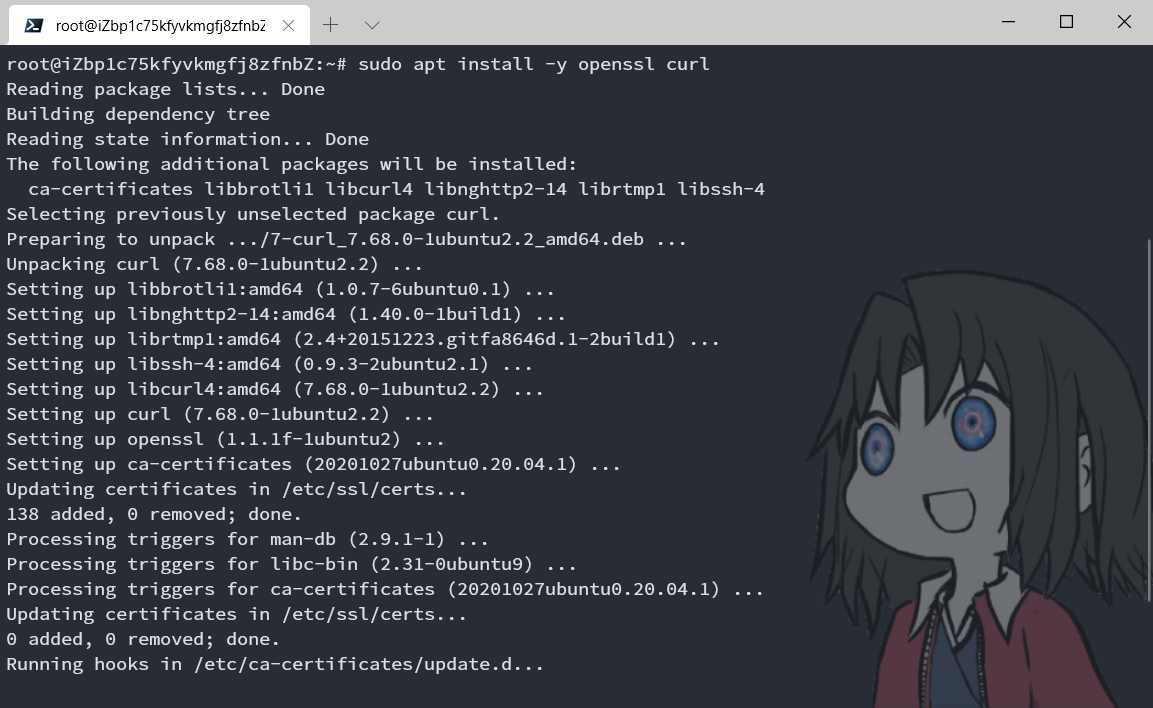
\includegraphics[width = 0.8 \textwidth]{curl.png}
            \caption{安装ubuntu依赖}
      \end{figure}

      \item 创建操作目录
      \begin{figure}[H]
            \centering
            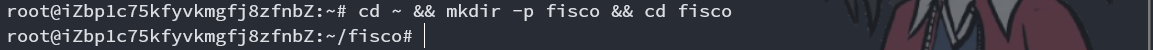
\includegraphics[width = 0.8 \textwidth]{fisco.png}
            \caption{创建操作目录}
      \end{figure}

      \item 下载build\_chain.sh脚本
      \begin{figure}[H]
            \centering
            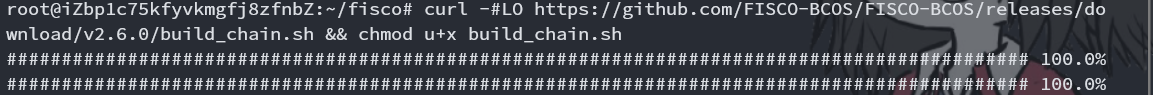
\includegraphics[width = 0.8 \textwidth]{build_chain.png}
            \caption{下载build\_chain.sh脚本}
      \end{figure}
\end{enumerate}

\subsubsection{搭建单群组4节点联盟链}
\begin{figure}[H]
      \centering
      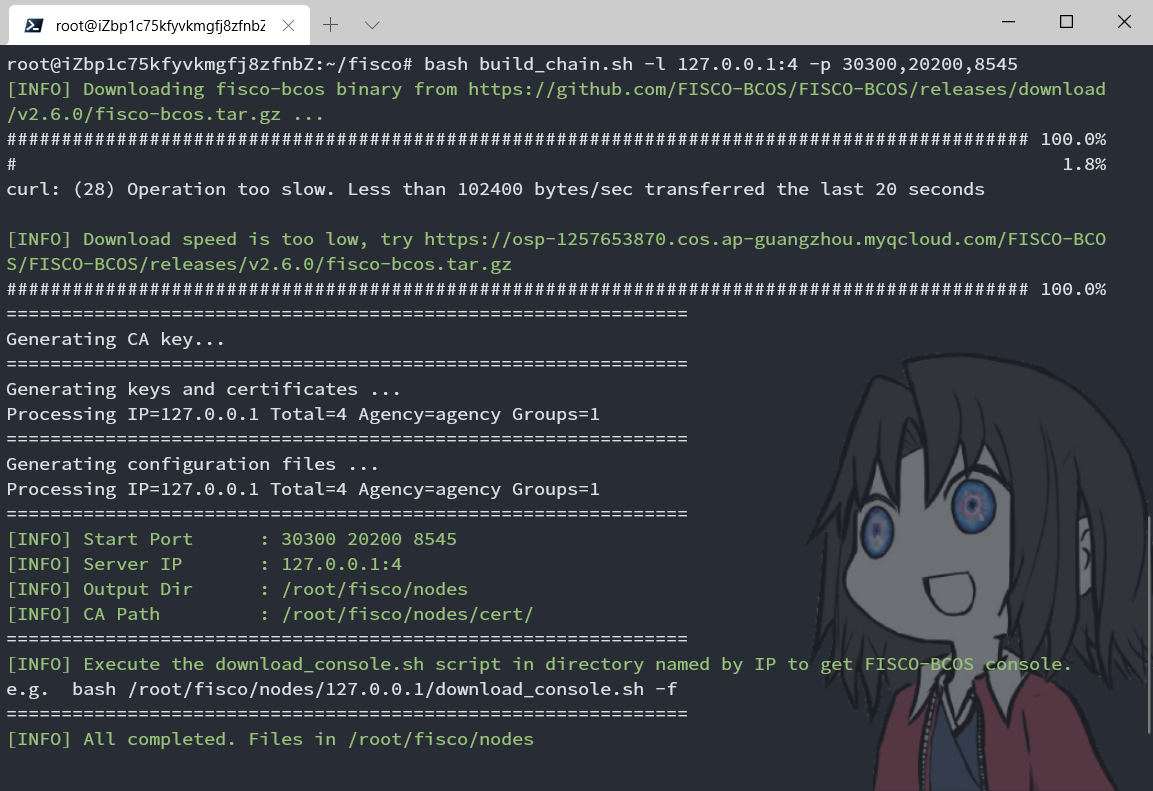
\includegraphics[width = 0.8 \textwidth]{nodes.png}
      \caption{搭建单群组4节点联盟链}
\end{figure}

\subsubsection{启动FISCO BCOS链}
\begin{figure}[H]
      \centering
      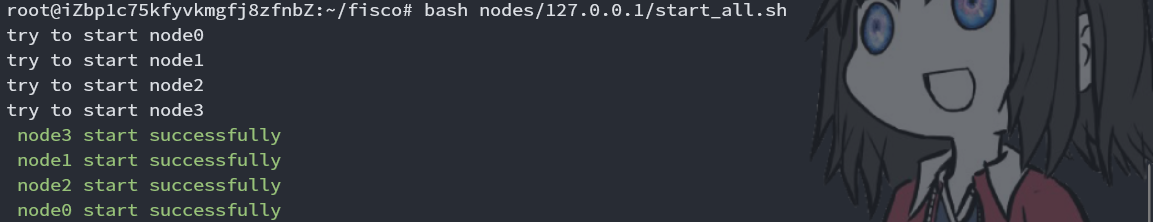
\includegraphics[width = 0.8 \textwidth]{start_all.png}
      \caption{启动FISCO BCOS链}
\end{figure}

\subsubsection{检查进程}
\begin{figure}[H]
      \centering
      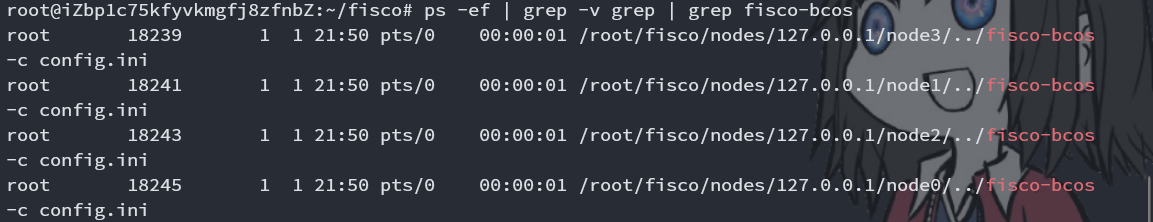
\includegraphics[width = 0.8 \textwidth]{ps.png}
      \caption{检查进程}
\end{figure}

\subsubsection{检查日志输出}
\begin{enumerate}
      \item 查看节点node0链接的节点数
      \begin{figure}[H]
            \centering
            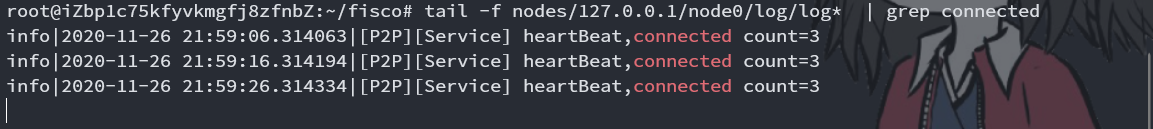
\includegraphics[width = 0.8 \textwidth]{connected.png}
            \caption{查看节点node0链接的节点数}
      \end{figure}

      \item 检查是否在共识
      \begin{figure}[H]
            \centering
            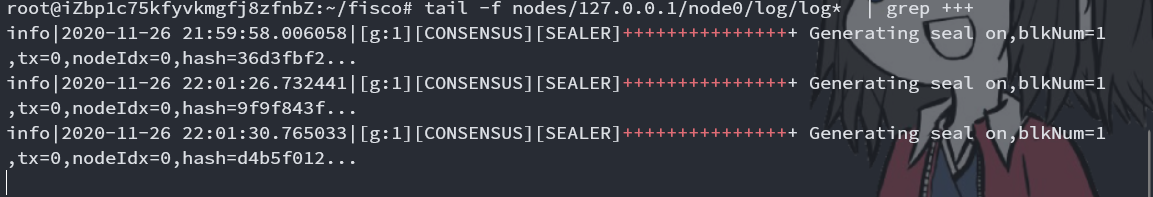
\includegraphics[width = 0.8 \textwidth]{+++.png}
            \caption{检查是否在共识}
      \end{figure}
\end{enumerate}

\subsection{配置及使用控制台}
\subsubsection{准备依赖}
\begin{enumerate}
      \item 安装java
      \begin{figure}[H]
            \centering
            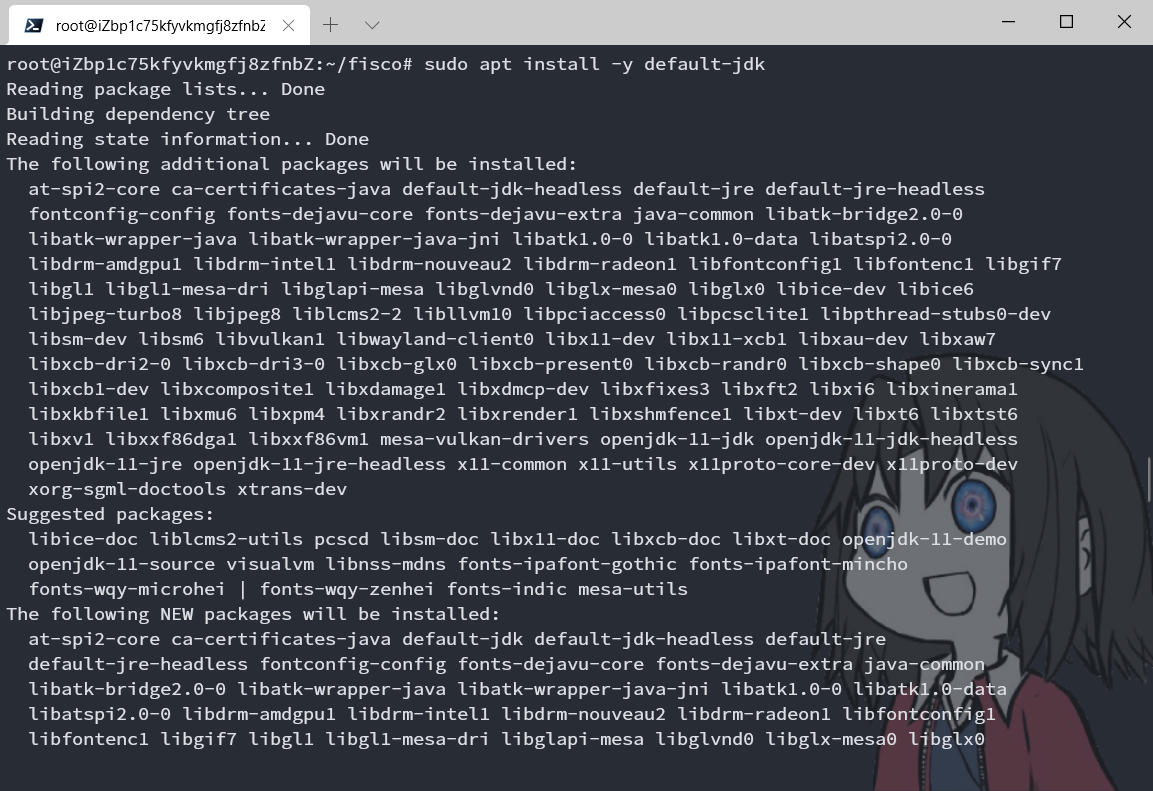
\includegraphics[width = 0.8 \textwidth]{java.png}
            \caption{安装java}
      \end{figure}

      \item 获取控制台并回到fisco目录
      \begin{figure}[H]
            \centering
            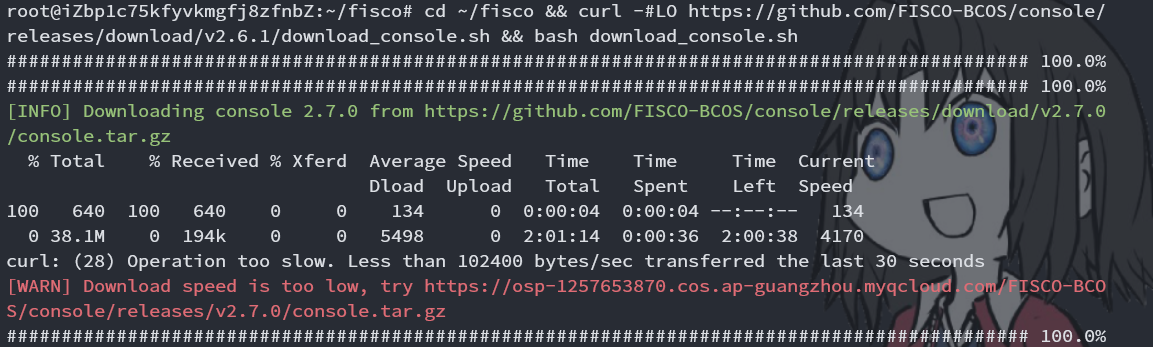
\includegraphics[width = 0.8 \textwidth]{console.png}
            \caption{获取控制台并回到fisco目录}
      \end{figure}

      \item 拷贝控制台配置文件
      \begin{figure}[H]
            \centering
            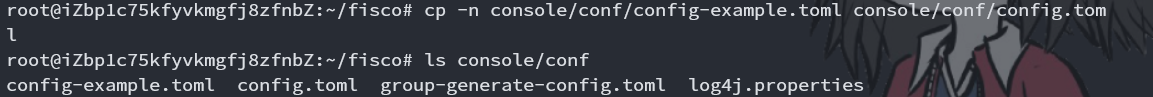
\includegraphics[width = 0.8 \textwidth]{cp.png}
            \caption{拷贝控制台配置文件}
      \end{figure}

      \item 配置控制台证书
      \begin{figure}[H]
            \centering
            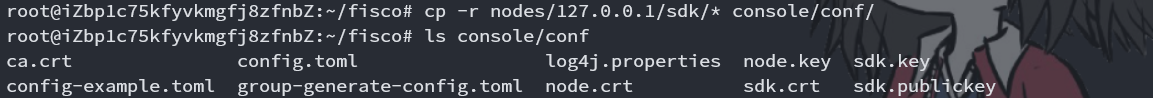
\includegraphics[width = 0.8 \textwidth]{sdk.png}
            \caption{配置控制台证书}
      \end{figure}
\end{enumerate}

\subsubsection{启动控制台}
\begin{figure}[H]
      \centering
      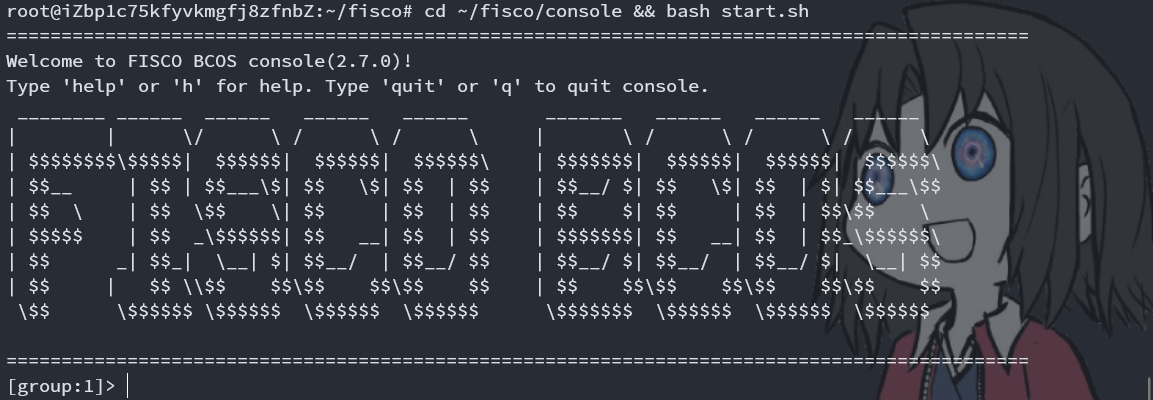
\includegraphics[width = 0.8 \textwidth]{start_console.png}
      \caption{启动控制台}
\end{figure}

\subsubsection{使用控制台获取信息}
\begin{enumerate}
      \item 获取客户端版本
      \begin{figure}[H]
            \centering
            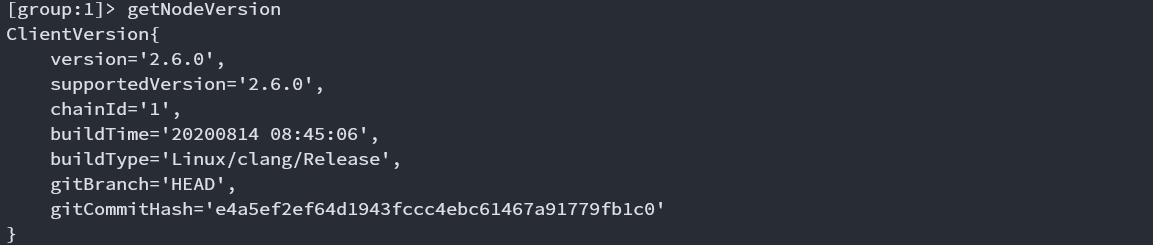
\includegraphics[width = 0.8 \textwidth]{version.png}
            \caption{获取客户端版本}
      \end{figure}

      \item 获取节点链接信息
      \begin{figure}[H]
            \centering
            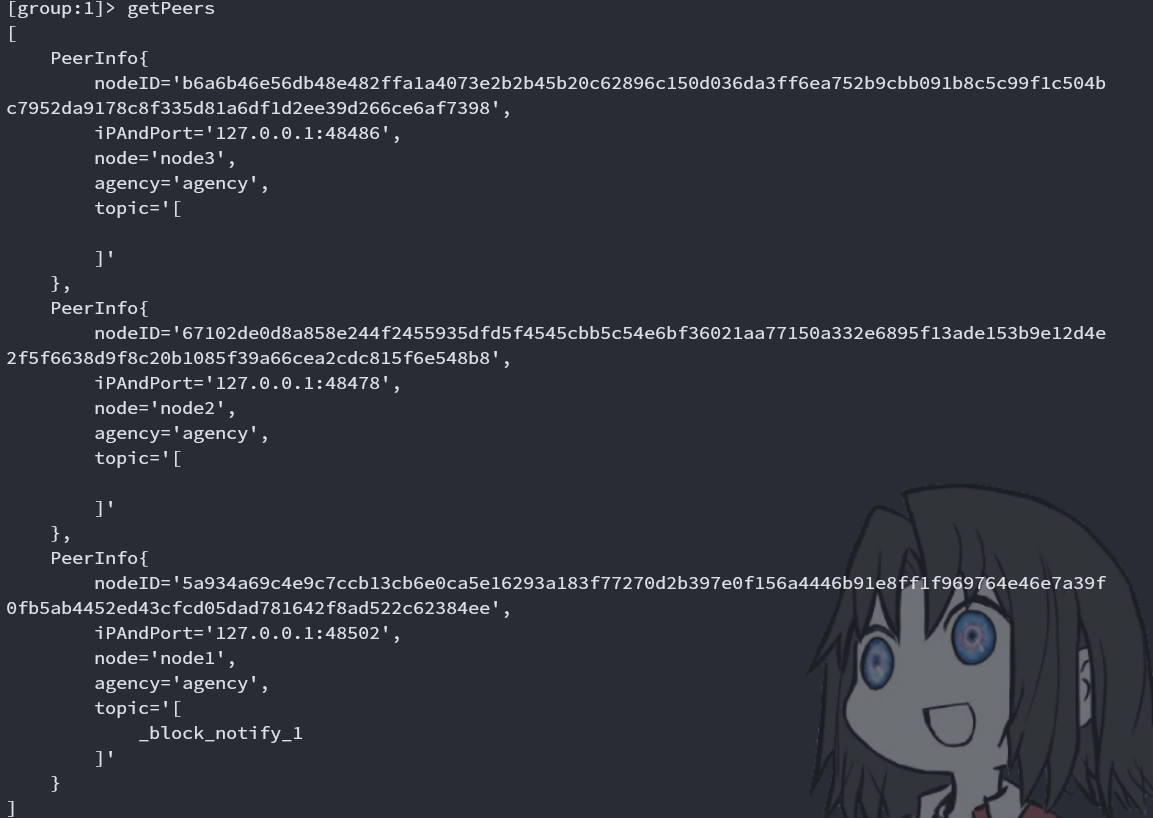
\includegraphics[width = 0.8 \textwidth]{peers.png}
            \caption{获取节点链接信息}
      \end{figure}
\end{enumerate}

\subsection{群组新增节点}
\subsubsection{为新节点生成私钥证书}
\begin{enumerate}
      \item 获取证书生成脚本
      \begin{figure}[H]
            \centering
            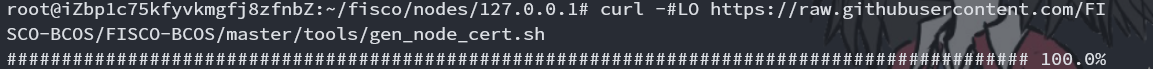
\includegraphics[width = 0.8 \textwidth]{gen_node.png}
            \caption{获取证书生成脚本}
      \end{figure}

      \item 生成新节点私钥证书
      \begin{figure}[H]
            \centering
            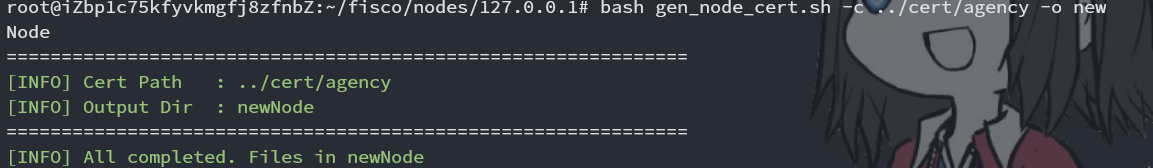
\includegraphics[width = 0.8 \textwidth]{newNode.png}
            \caption{生成新节点私钥证书}
      \end{figure}
\end{enumerate}

\subsubsection{准备配置文件}
\begin{enumerate}
      \item 拷贝群组1中节点node0配置文件与工具脚本
      \begin{figure}[H]
            \centering
            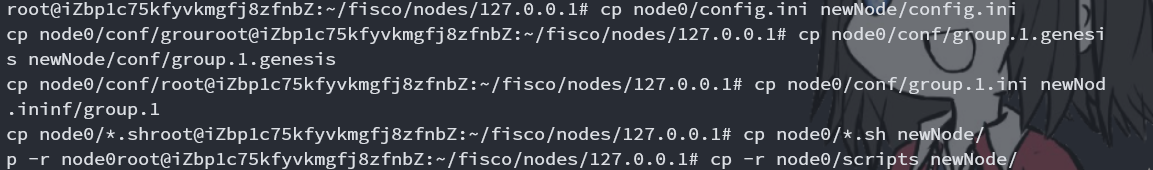
\includegraphics[width = 0.8 \textwidth]{cpnode0.png}
            \caption{拷贝群组1中节点node0配置文件与工具脚本}
      \end{figure}

      \item 更新newNode/config.ini中监听的IP和端口
      \begin{figure}[H]
            \centering
            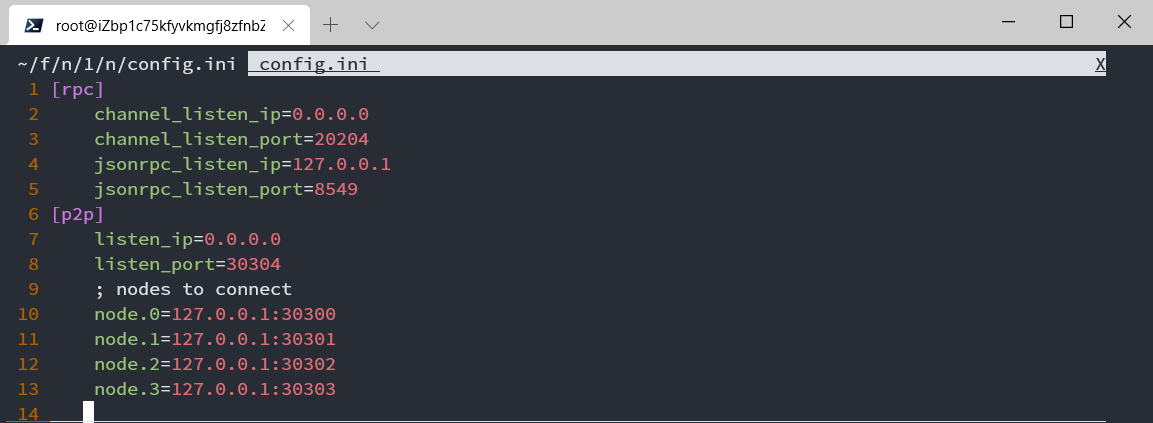
\includegraphics[width = 0.8 \textwidth]{config.png}
            \caption{更新newNode/config.ini中监听的IP和端口}
      \end{figure}

      \item 将新节点的P2P配置中的IP和Port加入原有节点的config.ini中的[p2p]字段
      \begin{figure}[H]
            \centering
            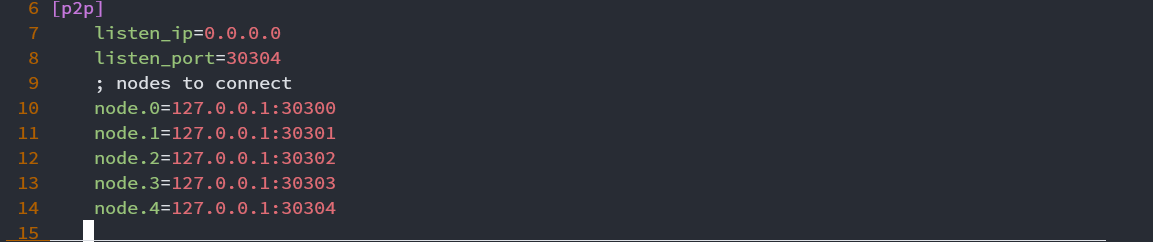
\includegraphics[width = 0.8 \textwidth]{newNodep2p.png}
            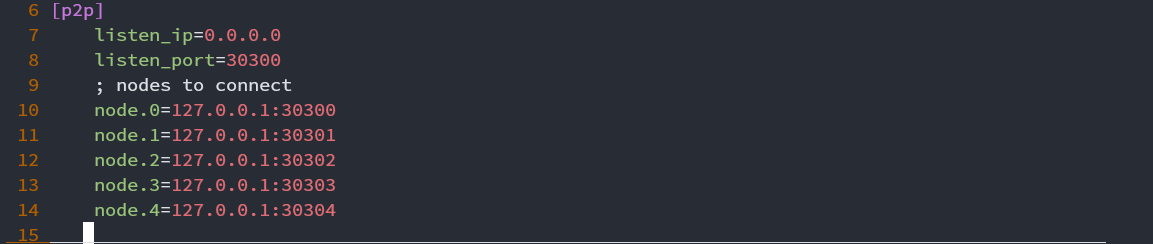
\includegraphics[width = 0.8 \textwidth]{node0p2p.png}
            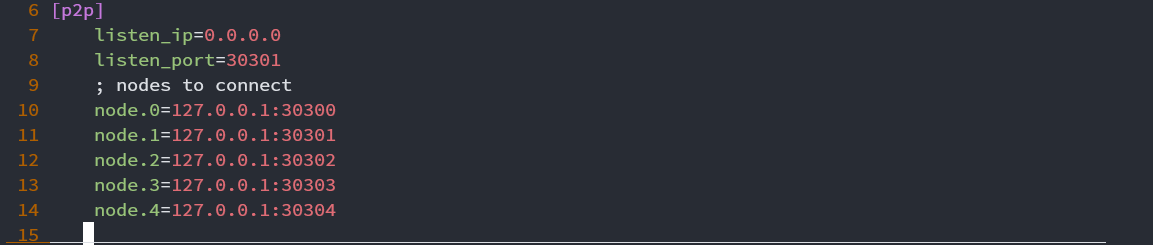
\includegraphics[width = 0.8 \textwidth]{node1p2p.png}
            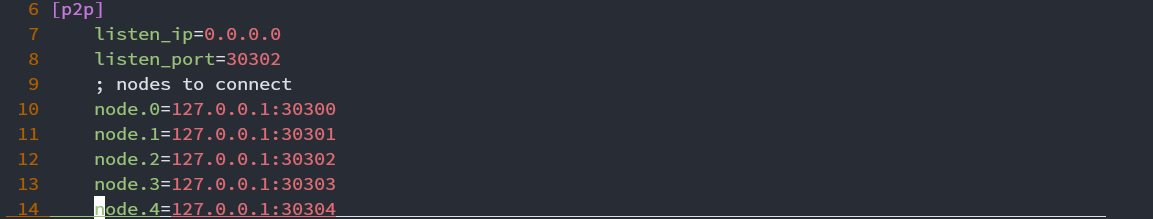
\includegraphics[width = 0.8 \textwidth]{node2p2p.png}
            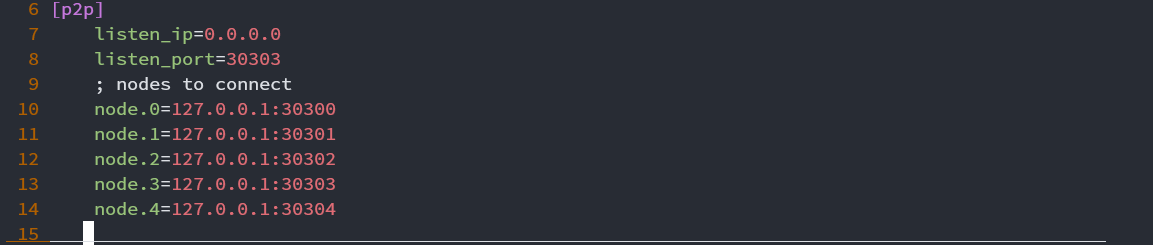
\includegraphics[width = 0.8 \textwidth]{node3p2p.png}
            \caption{将新节点的P2P配置中的IP和Port加入原有节点的config.ini中的[p2p]字段}
      \end{figure}
\end{enumerate}

\subsubsection{启动新节点并加入群组}
\begin{enumerate}
      \item 启动新节点,执行newNode/start.sh
      \begin{figure}[H]
            \centering
            
\includegraphics[width = 0.8 \textwidth]{startnewNode.png}
            \caption{启动新节点,执行newNode/start.sh}
      \end{figure}

      \item 通过console将新节点加入群组1
      \begin{figure}[H]
            \centering
            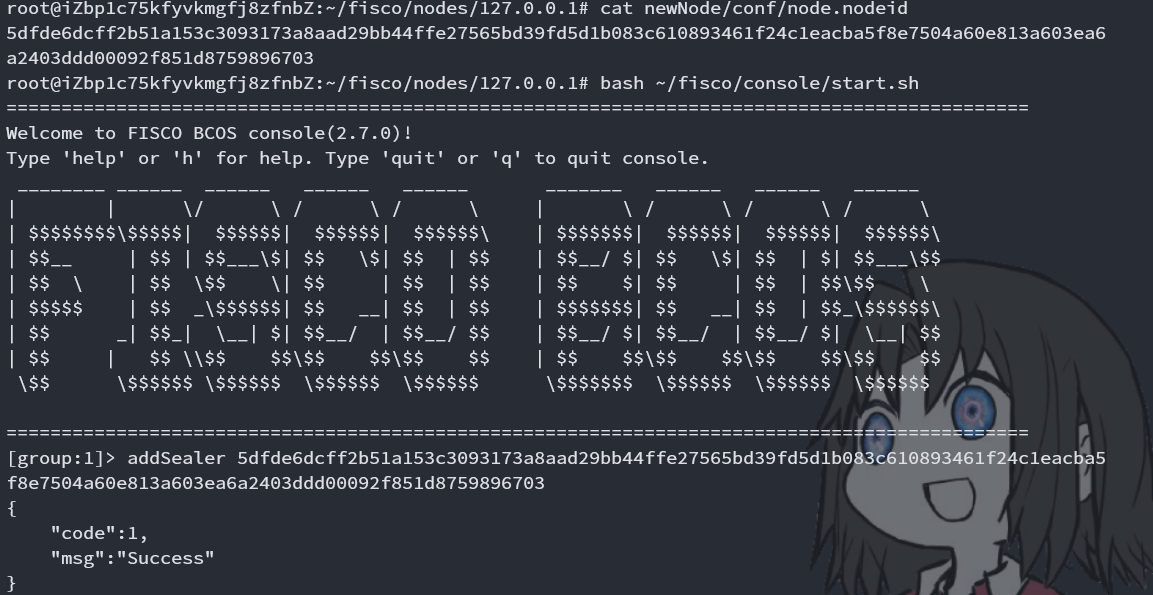
\includegraphics[width = 0.8 \textwidth]{addsealer.png}
            \caption{通过console将新节点加入群组1}
      \end{figure}

      \item 检查连接和共识
      \begin{figure}[H]
            \centering
            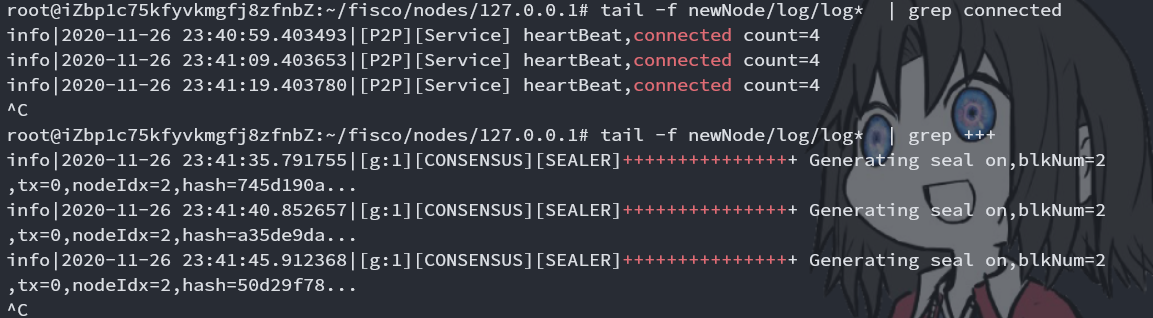
\includegraphics[width = 0.8 \textwidth]{checknewnode.png}
            \caption{检查连接和共识}
      \end{figure}
\end{enumerate}

\section{自行编写一个智能合约并部署到私有链上,同时完成合约调用。(截图说明部署流程)}
\subsection{Upvote合约}
\subsubsection{提供接口}
\begin{enumerate}
      \item \textbf{publish(content\_names)}:参数是内容名字的数组,发布内容,只有合约中唯一的发布者可以调用。
      \item \textbf{giveVotesToUser(user)}:参数是用户地址,给该用户10个点赞机会,只有合约中唯一的发布者可以调用,每个用户只能被授予1次。
      \item \textbf{upvote(name, votes)}:参数是内容名和点赞数,给某个内容点赞若干次。
      \item \textbf{winner()}:返回当前票数最高的内容名。
\end{enumerate}

\subsubsection{合约内容}
\begin{lstlisting}
pragma solidity>=0.4.24;

contract Upvote
{
    struct User
    {
        uint votes;
        bool given;
    }

    struct Content
    {
        string name;
        uint votes;
    }

    address public publisher;
    mapping(address => User) public users;
    Content[] public contents;

    constructor() public
    {
        publisher = msg.sender;
    }

    function publish(string memory name) public
    {
        require(msg.sender == publisher, "Only the publisher can publish contents.");
        for (uint i = 0; i < contents.length; i++)
        {
            require(keccak256(name) != keccak256(contents[i].name), "The content already exists.");
        }
        contents.push(Content({name: name, votes: 0}));
    }

    function giveVotesToUser(address user) public
    {
        require(msg.sender == publisher, "Only the publisher can give votes to a user.");
        require(users[user].given == false, "The user has been given votes.");
        users[user].votes = 10;
    }

    function upvote(string memory name, uint votes) public
    {
        User storage sender = users[msg.sender];
        require(sender.votes >= votes, "Don't have enough votes.");
        uint i = 0;
        for (; i < contents.length; i++)
        {
            if (keccak256(name) == keccak256(contents[i].name))
            {
                sender.votes -= votes;
                contents[i].votes += votes;
                break;
            }
        }
        require(i < contents.length, "The content doesn't exist.");
    }

    function winner() public view returns(string memory)
    {
        uint max_votes = 0;
        string storage name;
        for (uint i = 0; i < contents.length; i++)
        {
            if (max_votes < contents[i].votes)
            {
                max_votes = contents[i].votes;
                name = contents[i].name;
            }
        }
        return name;
    }
}
\end{lstlisting}

\subsection{部署Upvote合约}
\begin{figure}[H]
      \centering
      
\includegraphics[width = 0.8 \textwidth]{deploy.png}
      \caption{部署Upvote合约}
\end{figure}


\subsection{调用Upvote合约}
\subsubsection{创建2个新的账户}
      \begin{figure}[H]
            \centering
            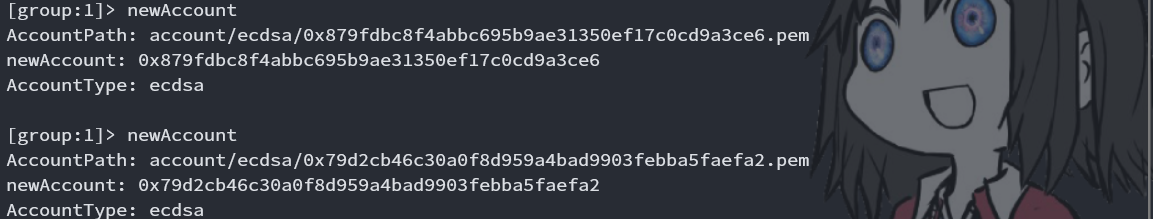
\includegraphics[width = 0.8 \textwidth]{newAccount.png}
            \caption{创建2个新的账户}
      \end{figure}
\subsubsection{调用Upvote合约的接口}
\begin{enumerate}
      \item 使用当前新用户调用giveVotesToUser,失败
      \begin{figure}[H]
            \centering
            
\includegraphics[width = 0.8 \textwidth]{giveVotesError.png}
            \caption{使用当前新用户调用giveVotesToUser}
      \end{figure}

      \item 使用部署合约用户调用giveVotesToUser,成功,说明部署合约的用户是publisher。
      \begin{figure}[H]
            \centering
            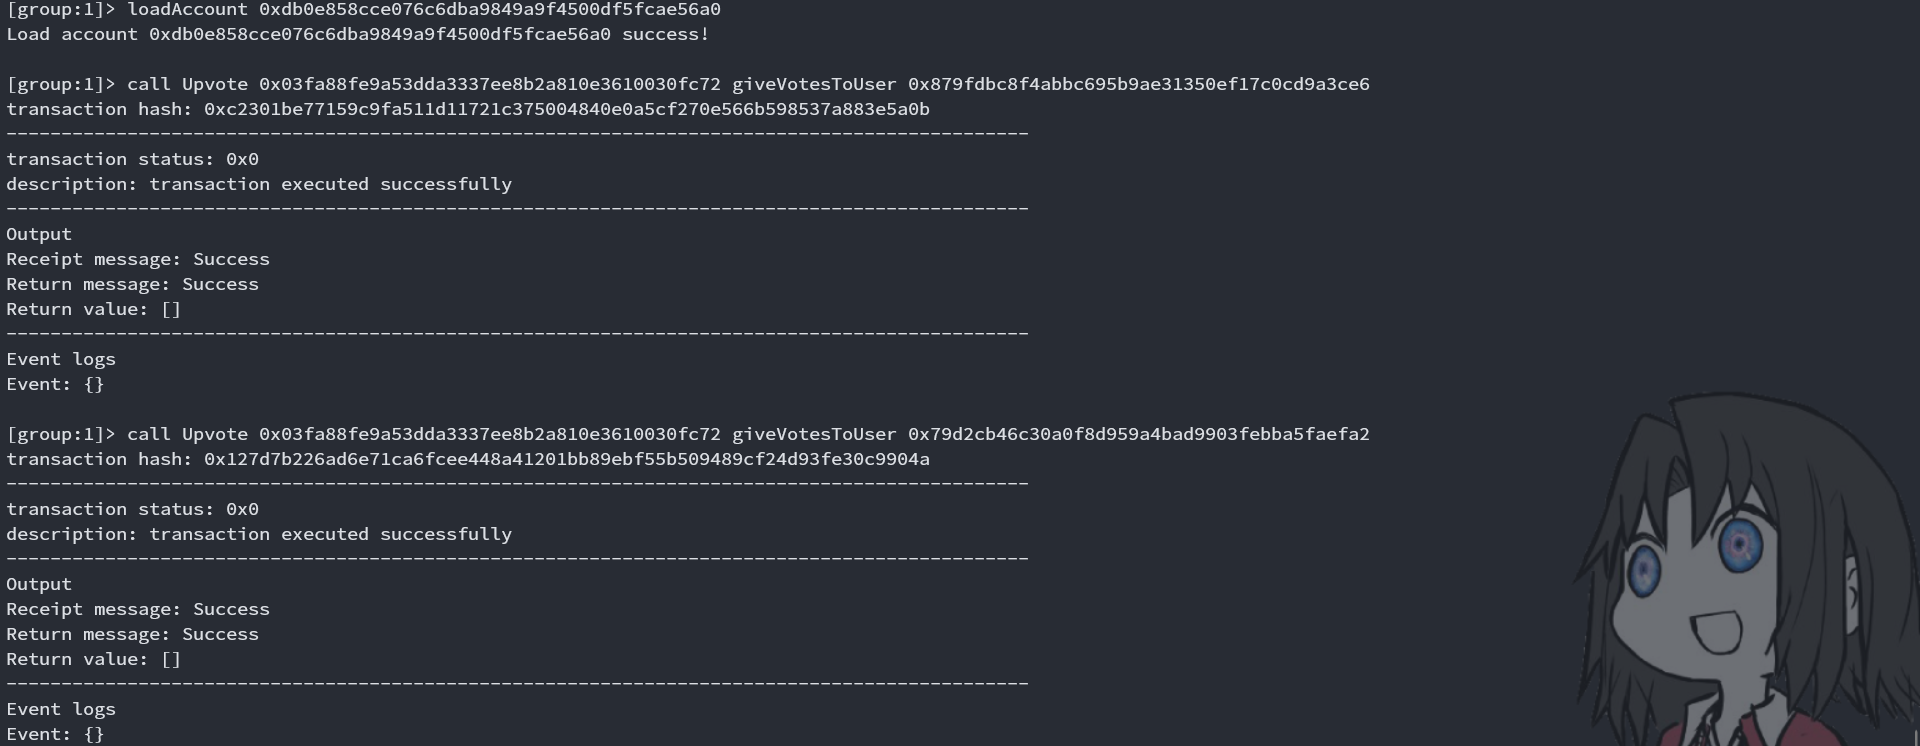
\includegraphics[width = 0.8 \textwidth]{giveVotes.png}
            \caption{使用部署合约用户调用giveVotesToUser}
      \end{figure}

      \item publisher调用publish,如果遇到相同内容会报错
      \begin{figure}[H]
            \centering
            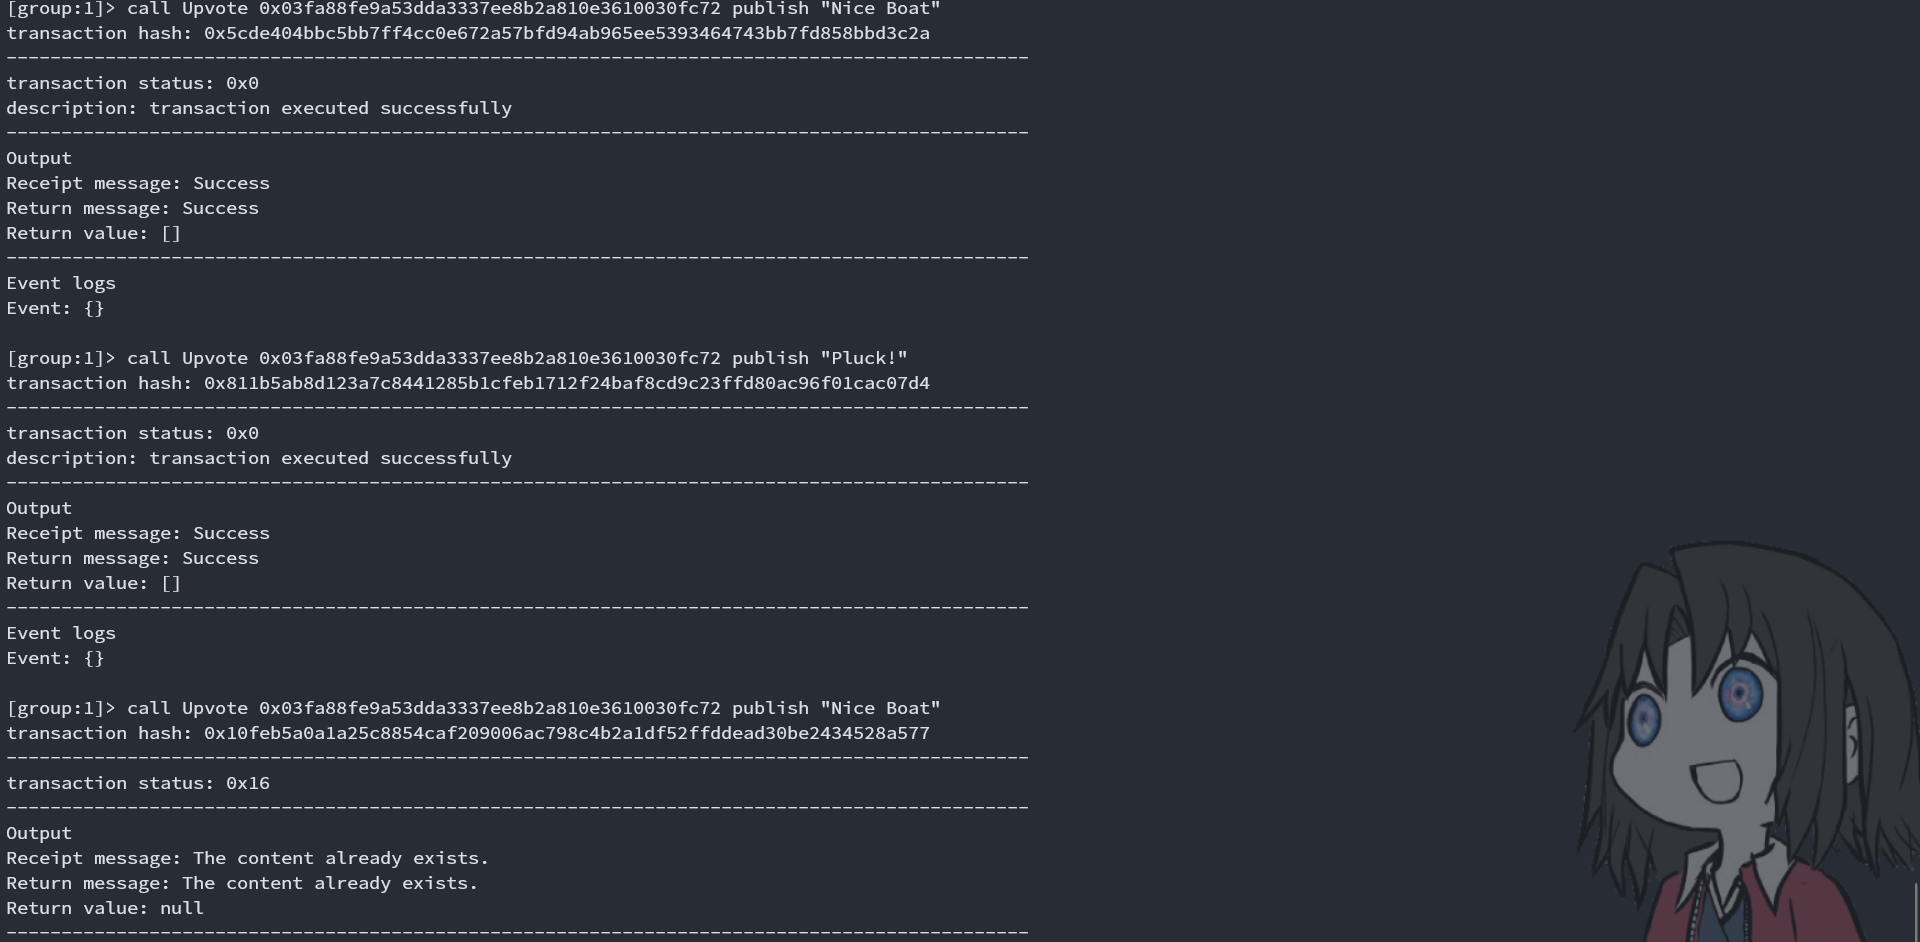
\includegraphics[width = 0.8 \textwidth]{publish.png}
            \caption{publisher调用publish}
      \end{figure}

      \item 切换用户调用upvote
      \begin{itemize}
            \item 当票数足够时,成功运行
            \begin{figure}[H]
                  \centering
                  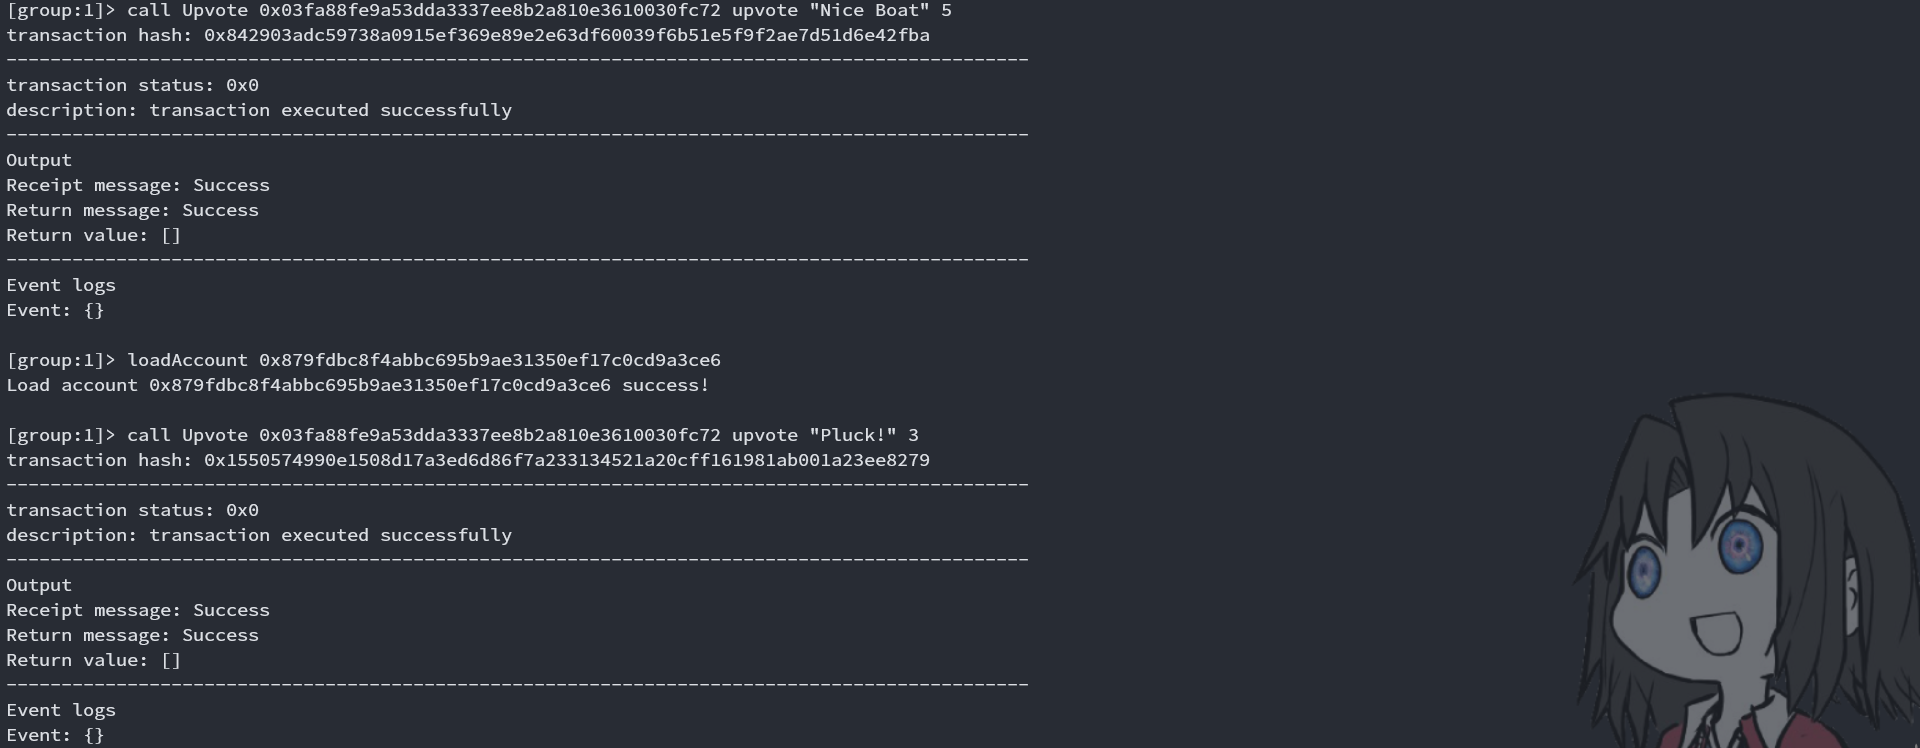
\includegraphics[width = 0.8 \textwidth]{upvote.png}
                  \caption{调用upvote票数足够}
            \end{figure}

            \item 当票数不够时,报错
            \begin{figure}[H]
                  \centering
                  
\includegraphics[width = 0.8 \textwidth]{upvoteerror.png}
                  \caption{调用upvote票数不够}
            \end{figure}
      \end{itemize}

      \item 调用winner
      \begin{figure}[H]
            \centering
            
\includegraphics[width = 0.8 \textwidth]{winner.png}
            \caption{调用winner}
      \end{figure}
\end{enumerate}

\section{使用命令查看一个区块,并对各个字段进行解释。}
\begin{figure}[H]
      \centering
      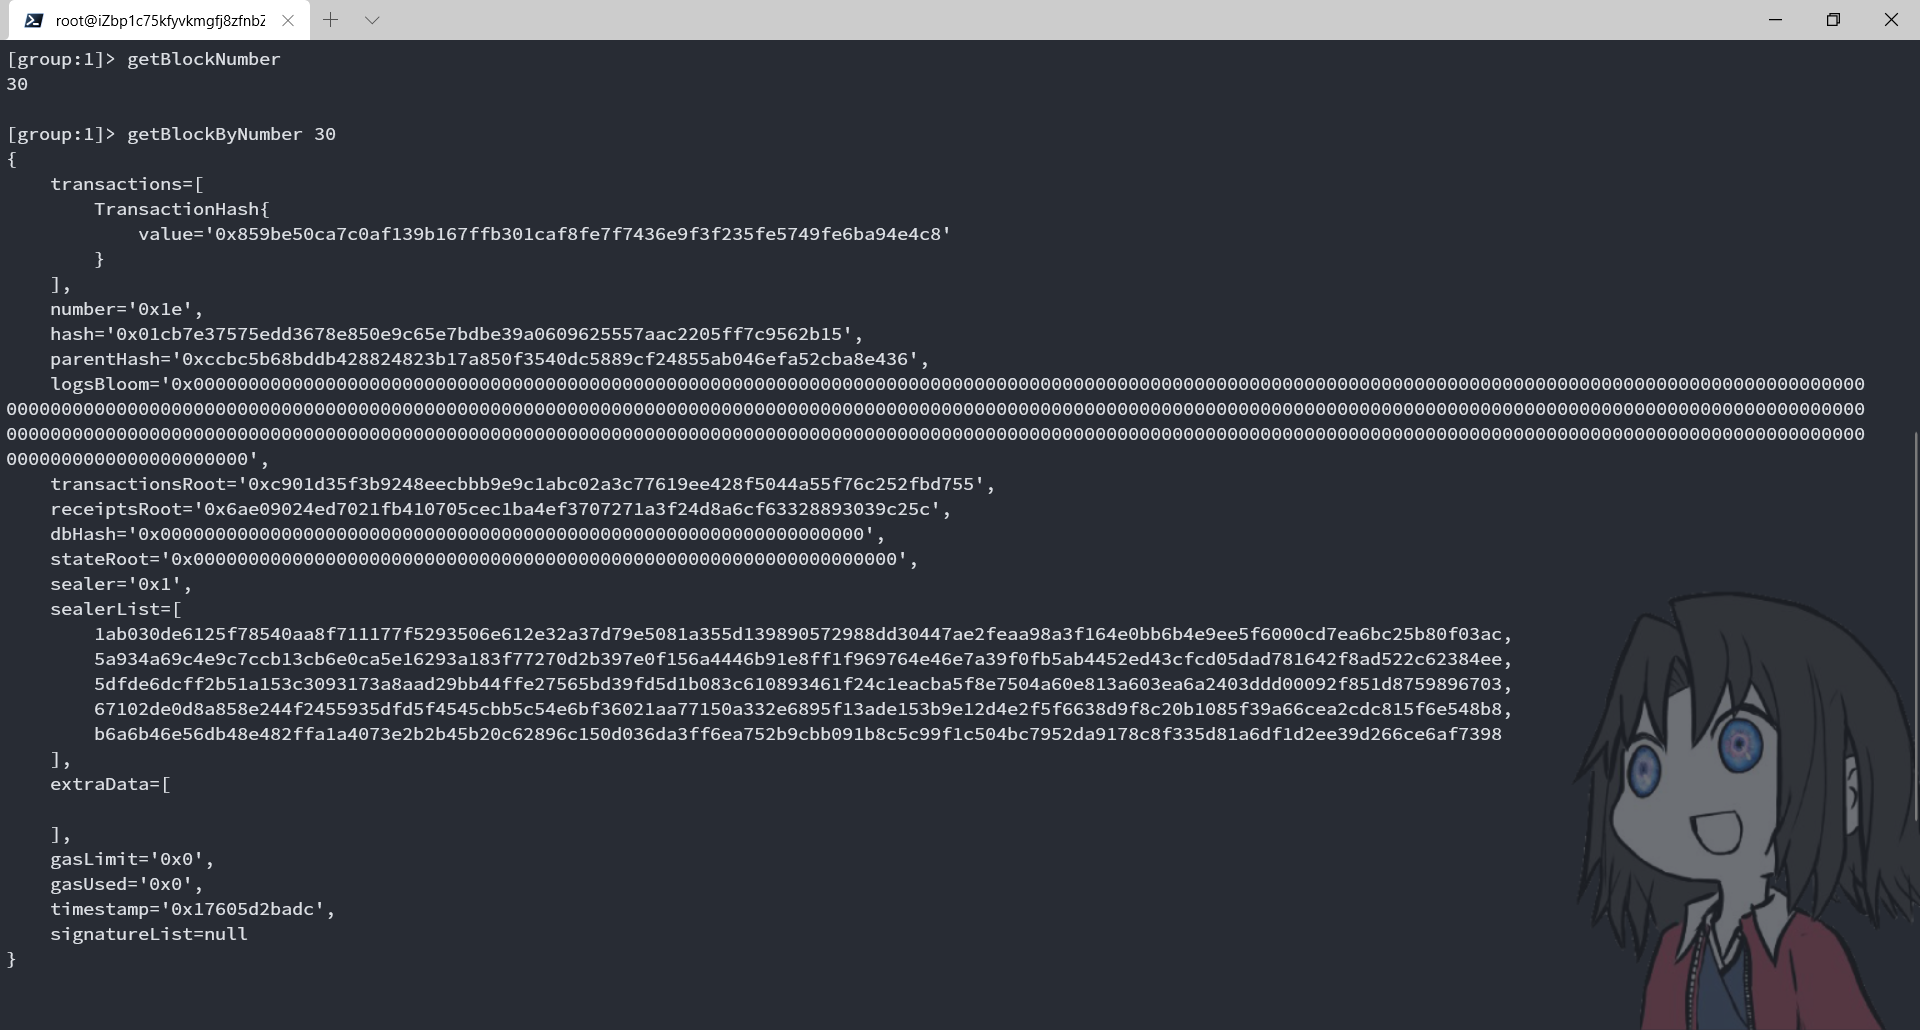
\includegraphics[width = 0.8 \textwidth]{block.png}
      \caption{调用upvote票数不够}
\end{figure}
\begin{itemize}
      \item transactions:交易列表
      \begin{itemize}
            \item TransactionHash:交易哈希
      \end{itemize}
      \item number:区块高度
      \item hash:区块哈希
      \item parentHash:父区块哈希
      \item logsBloom:log的布隆过滤器值
      \item transactionRoot:区块内所有交易的merkle根
      \item receiptsRoot:区块内所有交易回执的merkle根
      \item dbHash:记录交易数据变更的哈希
      \item stateRoot:状态根哈希
      \item sealer:共识节点序号
      \item sealerList:共识节点列表
      \item extraData:交易内的extraData
      \item gasLimit:区块中允许的gas最大值
      \item gasUsed:区块中所有交易消耗的gas
      \item timestamp:时间戳,单位毫秒
      \item signatureList:PBFT共识的签名列表
\end{itemize}
\end{document}